\chapter{Sensibility analysis of optimal investment times}
\label{chapter:stoptime}



%%%%%%%%%%%%%%%%%%%%%%%%%%%%%%%%%%%%%%%%%%%%%%%%%%%%%%%%%%%%%%%%%%%%%%%%
\section{Introduction}
\label{section:stoptime_intro}

In this section we will analyse the optimal times to invest regarding the three different models developed on previous sections.

First, we will analyse some estimated relevant measures - such as mean, median and standard deviation - of the optimal investment times, by considering different demand initial values.

Secondly, we will analyse how the estimated mean of optimal investment times behaves with volatility and compare their behaviour with the change on associated threshold value and optimal capacity level.

\section{Initial demand values $x_0$}

\subsubsection{Methodology}

We start by fixing vaues regarding the relevant parameters to each of the models, with the exception of the initial point $x_0$, that we will vary here.

Regarding the first and second models, discussed on Chapters \ref{chapter:1} and \ref{chapter:2}, respectively, we consider $x_0 \in [0.0002, 3 \times  \texttt{xStep} + \lfloor \max{ \{ x_B^*, x_C^* \} } \rfloor]  ]$, this is, values $x_{0_i}$ which are incremented $i$-th times by \texttt{xStep}=0.0002. Due to the noticeable difference of the order of magnitude of the thresholds on Chapter \ref{chapter:3}, we consider the interval of possible initial values to be $[0.002, 10 \times \texttt{xStep} +  \lfloor  x_{1,A}^* \rfloor] ]$, in particular, values $x_{0_i}$ which are incremented $i$-th times \texttt{xStep}=0.002.
		
By fixing the firm's situation to analyse, we fix as well the respective demand threshold, for which, higher demand values, state that the investment should be done.

Therefore we execute the function \texttt{generalStopTime}, that given the extremes of the domain of initial points to be considered, it simulates \texttt{NsamplePaths}=1000 demand sample paths, until they all reach the threshold chosen. It returns as output the set of times corresponding to when each sample path reached the referred threshold.
After that, per each initial value $x_{0_i}$, we calculate the respective measure of interest (mean, median or standard deviation), whose result is presented in plots, as can be seen in the section hereunder.

Note that, since this is a mere illustration of the models deduced, for following results we consider a \texttt{timeStep}=1. However this value can be changed and chosen to be in the same time scale as the estimated drift $\mu$ and volatility $\sigma$ of the GBM or regarding a certain time window. 


\subsubsection{Results}

Regarding models derived on Sections \ref{chapter:1} and \ref{chapter:2}, the following set of parameters was considered:
\begin{table*}[!htb]
	\centering
	\begin{tabular}{lllllll}
		$\bullet$ & $\mu=0.03$     &  & \hspace{7cm} &  &  $\bullet$ & $\alpha=0.01$ \\
		$\bullet$ & $\sigma=0.1$ &  & \hspace{7cm} &  &  $\bullet$ & $\theta=10$   \\
		$\bullet$ & $r=0.05$       &  & \hspace{7cm} &  &  $\bullet$ & $K_0=90$       \\
		$\bullet$ & $\delta=2$     &  & \hspace{7cm} & &  $\bullet$ & $K_1=100$  	\\                                
	\end{tabular}
	%\caption{bjde}
\end{table*}
Despite $\sigma$, these are the same values used in Sections \ref{chapter:1} and \ref{chapter:2}.

Regarding the model derived on Section \ref{chapter:3}, the following set of parameters was considered:
\begin{table*}[!htb]
	\centering
	\begin{tabular}{lllllll}
		$\bullet$ & $\mu=0.45$     &  & \hspace{7cm} &  &  $\bullet$ & $\alpha=0.015$ \\
		$\bullet$ & $\sigma=0.1$ &  & \hspace{7cm} &  &  $\bullet$ & $\theta=1.5$   \\
		$\bullet$ & $r=0.85$       &  & \hspace{7cm} &  &  $\bullet$ & $K_0=51.5$       \\
		$\bullet$ & $\delta=0.95$     &  & \hspace{7cm} & &  $\bullet$ & $K_1=2.5$  		\\
		$\bullet$ & $\eta=0.007$.     
	\end{tabular}
\end{table*}

Despite $\sigma$, these are the same values used on Chapter \ref{chapter:3}. Note that by choosing $\eta=0.007$, we have that $\eta< \eta^*$ and thus we are in the situation where the firm has two decisions to make: when it should invest and start the simultaneous production; when it should stop  the simultaneous production and produce solely the \textit{new} product.
On Figure \ref{fig:stoptime_1} we can find the results obtained.

Note that, in which of the plots, there is represented a dashed line corresponding to the demand threshold level for which the firm should make its investment decision. As expected, for any initial value higher than the threshold,
% there is no waiting time until it's optimal to make the investment decision 
the firm is not expected to wait to decide
- not only the mean and median are null, so it is the standard deviation.


Observe that the smaller the initial value $x_0$, the higher (all) its respective measures are. 

Also, the higher threshold level, the longer (in average and median) the firm will need to wait until it should invest. This situation is particularly noticeable on results regarding Chapter \ref{chapter:1}.

The results concerning the mean and the median of the optimal investment times have an intuitive explanation: when starting with a small demand level (or considering an higher threshold), one expects to wait more time until the demand level reaches the threshold demand level, than when starting with an higher level (or with a smaller threshold). However the result concerning the standard deviation is not that obvious. It can arise due to the randomness of the GBM and its time increasing variance, respectively given by $Var(X_t)=X_0^2 e^{2\mu t}(e^{\sigma^2 t} -1), \ \forall t\geq0, \mu \geq 0$, which allows the sample path to be more diverse (either in observed states as in running lenght) and thus obtain also more distinct stopping times.
%Also, observe that for higher threshold levels, in average and median, the firm will need to wait more time until it is able to invest. This fact is particularly noticeable on the first two rows, whose results are taken with respect to the first situation (Section \ref{chapter:1}).
\pagebreak

\begin{figure}[!ht]
	\begin{subfigmatrix}{6}
		\subfigure[Mean \& Median of $\tau_B^*$ w.r.t. \eqref{eq:sistema} ]{\includegraphics[width=0.35\textwidth]{StopTime/1_BMtau.pdf}}
		\subfigure[Standard Deviation of $\tau_B^*$ w.r.t. \eqref{eq:sistema} ]{\includegraphics[width=0.35\textwidth]{StopTime/1_BMsd.pdf}}
		\subfigure[Mean \& Median of $\tau_C^*$ w.r.t. \eqref{eq:prob1_xC}]{\includegraphics[width=0.35\textwidth]{StopTime/1_COMtau.pdf}}
		\subfigure[Standard Deviation of $\tau_C^*$ w.r.t. \eqref{eq:prob1_xC}]{\includegraphics[width=0.35\textwidth]{StopTime/1_COMsd.pdf}}
		\subfigure[Mean \& Median of $\tau_B^*$ w.r.t. \eqref{2_xB} ]{\includegraphics[width=0.35\textwidth]{StopTime/2_BMtau.pdf}}
		\subfigure[Standard Deviation of $\tau_B^*$ w.r.t. \eqref{2_xB} ]{\includegraphics[width=0.35\textwidth]{StopTime/2_BMsd.pdf}}
		\subfigure[Mean \& Median of $\tau_C^*$ w.r.t. \eqref{eq:prob2_xC} ]{\includegraphics[width=0.35\textwidth]{StopTime/2_COMtau.pdf}}
		\subfigure[Standard Deviation of $\tau_C^*$ w.r.t. \eqref{eq:prob2_xC} ]{\includegraphics[width=0.35\textwidth]{StopTime/2_COMsd.pdf}}
		\subfigure[Mean \& Median of $\tau_{1,A}^*$ w.r.t. \eqref{eq:3_x1A}]{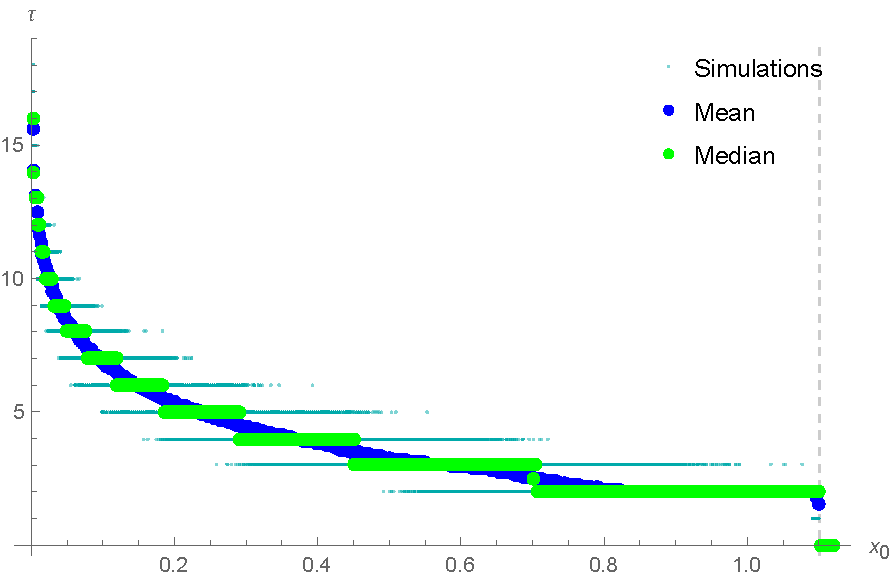
\includegraphics[width=0.35\textwidth]{StopTime/3_BMtau.pdf}}
		\subfigure[Standard Deviation of $\tau_{1,A}^*$ w.r.t. \eqref{eq:3_x1A} ]{\includegraphics[width=0.35\textwidth]{StopTime/3_BMsd.pdf}}
	\end{subfigmatrix}
	\caption{Sensibility analysis of estimated mean and median (leftmost column) and standard deviation (rigthmost column) of the optimal investment time for each of the three situations studied, regarding different initial values $x_0$.}
	\label{fig:stoptime_1}
\end{figure}

We highlight here, as well, the fact that the mean and the median of investment times is approximately equal, suggesting that the distribution of investment times is approximately symmetric.

On the last row we find the results concerning the optimal time to invest in a \textit{new} product and start to produce, simultaneously, the \textit{old} and \textit{new} products, as studied on Section \ref{chapter:3}. This result appears to be sparser (regarding the median) and more oscillated (regarding the standard deviation) than the others, due to the raise on the increment of the initial value (\texttt{xStep}), while the range of waiting times metrics isn't as wide as the ones obtained on previous situations. This might be seen also as a \textit{zoom} of the behaviour presented on previous plots.


Now, regarding the optimal time to stop the production of the established product, studied on Chapter \ref{chapter:3}, we obtain results presented on Table \ref{stoptime_t}.
\begin{table}[!htb]
	\caption{Sensibility analysis of estimated mean, median and standard deviation of optimal time to decide stop the production of the established product when considering an observed demand $x_{1,A}^*$.}
	\centering
	\begin{tabular}{ccc}
		Mean & Median & Standard Deviation \\ \hline
		5.49 & 5.00 & 0.77
	\end{tabular}
\label{stoptime_t}
\end{table}

Here we only consider the demand process to start at $x_{1,A}^*$, since this is the instant after which we are able to make the mentioned decision. Therefore, mean and median are taken considering as \textit{initial instant} the time at which the firm decides to invest in the new product and start the simultaneous production, that is, $\tau^*_{1,A}=\inf \{ t\geq 0: X_t \geq x^*_{1,A} \}$. Thus, the mean/median presented should be read as the mean/median time after the investment on the \textit{new} product was done. To obtain the estimated mean/median time for which the firm produces solely the \textit{new} product, one should add the value presented on Table \ref{stoptime_t} to the one obtained as the mean/median time to invest in the \textit{new} product, for a given initial demand value $x_0$.    

We obtain similar results as the ones stated above, in particular, that the mean and median of investment times is similar, suggesting that they have a symmetric distribution.


\section{Volatility sensibility analysis}

In this section we are interested to observe how optimal investment times behave with volatility.

\subsubsection{Methodology}

The results are mainly obtained recurring to function \texttt{estTau}, which has function \texttt{stopTimemod} included.

Considering a model and respective parameters fixed, \texttt{stopTimemod} simulates \texttt{NsamplePaths}=100 demand sample paths, recording the instant at each of them either reaches the demand threshold considered or reaches time \texttt{horizon}. Since it's not deterministic that all sample paths will reach the threshold, this last condition is crucial to assure that the algorithm runs in \textit{human-time}. On the results showed hereunder we consider \texttt{horizon}=1000 time units.

Function \texttt{estTau} calculates the mean of the investment times obtained by \texttt{stopTimemod} per each volatility level $\sigma_i$, which starts in 0.01 and it is incremented $i$-th times 0.01, until reaches \texttt{$\sigma$ Max}=0.5, that is $\sigma_i=0.01+i \times 0.01 \in [0.01,0.5]$.

We run \texttt{estTau} for each of the models studied - either benchmark or capacity optimization model - and considering two initial points $x_0 \in \{0.001, \ 0.01 \}$. We also evaluate as well the respective threshold values and optimal capacity in order to compare results obtained.




\subsubsection{Results}

Despite the initial demand value and volatility, the set of parameters considered, regarding each model, was the same as chosen in the previous section. We consider here as well a \texttt{timeStep} of one time unit. For each of the three situations studied, we present the graphical result and a table in which are numerically presented the diverse measures analysed regarding volatility increments of 0.05.

$\bullet$ \textbf{Situation on Chapter \ref{chapter:1}: firm has no products in the market and wants to introduce a new one}

On Figure \ref{fig:vol_1} we observe that both optimal investment times have a non-monotonic behaviour with the volatility. Even when the threshold level and the optimal capacity level increase with it.

One can also note that the optimal investment times for both benchmark and capacity optimization models increase significantly for volatilities $\sigma>0.35$. This effect is more significant when considering a smaller initial value $x_0$.

\begin{figure}[!ht]
	\begin{subfigmatrix}{3}
		\subfigure[(Estimated) mean of optimal investment times. ]{\includegraphics[width=0.32\textwidth]{StopTime/1_meantau.pdf}}
		\subfigure[Demand threshold. ]{\includegraphics[width=0.32\textwidth]{StopTime/1_x.pdf}}
		\subfigure[Optimal capacity level.]{\includegraphics[width=0.32\textwidth]{StopTime/1_k.pdf}}
	\end{subfigmatrix}
	\caption{Sensibility analysis of the (estimated) mean of optimal investment time, the threshold level and the optimal capacity level (referred on Chapter \ref{chapter:1}) with the volatility, regarding different initial values $x_0 \in \{0.001, \ 0.01\}$.}
	\label{fig:vol_1}
\end{figure}

Besides previous conclusions, on Table \ref{tab:vol_1}, we observe that the difference between $\tau_B^*$ and $\tau_C^*$, for $x_0=0.01$, is more noticeable than what it seems in Figure \ref{fig:vol_1}.

We found no relation between the behaviour of optimal investing times and threshold levels or optimal capacity. However it seems to exist an optimal volatility level such that the optimal investment time is the lowest. In this case, this optimal volatility level $\sigma^*$ seems to be $0.15 < \sigma^* < 0.25$ for $x_0=0.001$ and $\sigma^*<0.15$ for $x_0=0.01$.

\begin{table}[!ht]
	\centering
	\caption{Sensibility analysis of the (estimated) mean of optimal investment time, the threshold level and the optimal capacity level (referred on Chapter \ref{chapter:1}) with the volatility, regarding different initial values $x_0 \in \{0.001, \ 0.01\}$.}
	\begin{tabular}{c|ccccccccl}
		\hline
		\text{ $\sigma $ } & 0.05 & 0.1 & 0.15 & 0.2 & 0.25 & 0.3 & 0.35 & 0.4 \\ \hline
		$K^*$ & 381.04 & 395.08 & 410.92 & 425.39 & 437.62 & 447.66 & 455.80 & 462.41 \\
		$x_B^*$ & 0.012 & 0.013 & 0.015 & 0.017 & 0.020 & 0.023 & 0.027 & 0.032 \\
		$x_C^*$ & 0.017 & 0.019 & 0.022 & 0.027 & 0.032 & 0.038 & 0.045 & 0.053 \\ \hline
	   $\overline{\tau _B}$ & 68.36 & 58.75 & 53.82 & 51.59 & 53.81 & 52.89 & 65.64 & 85.33 & \rdelim\}{2}{0.05mm}[$x_0=0.001$]  \\
		$\overline{\tau _C}$ & 77.99 & 70.06 & 65.51 & 64.65 & 66.83 & 66.16 & 82.85 & 165.11 \\ \hline
		$\overline{\tau _B}$ & 4.41 & 5.03 & 6.69 & 7.4 & 8.77 & 11.44 & 10.66 & 12.02 &	\rdelim\}{2}{0.05mm}[$x_0=0.01$] \\
		$\overline{\tau _C}$ & 13.73 & 12.82 & 13.64 & 14.35 & 15.36 & 17.2 & 19.92 & 22.24 \\ \hline
	\end{tabular}
\label{tab:vol_1}
\end{table}



\pagebreak

$\bullet$ \textbf{Situation on Section \ref{chapter:2}: firm has an established product and want to introduce a new one, replacing the other one}


On Figure \ref{fig:vol_2} we can observe that conclusions stated before hold. Optimal investment times have a non-monotonic behaviour with the volatility and they seem not to be related neither with threshold values or the optimal capacity level. 

\begin{figure}[!ht]
	\begin{subfigmatrix}{3}
		\subfigure[(Estimated) mean of optimal investment times. ]{\includegraphics[width=0.32\textwidth]{StopTime/2_meantau.pdf}}
		\subfigure[Demand threshold. ]{\includegraphics[width=0.32\textwidth]{StopTime/2_x.pdf}}
		\subfigure[Optimal capacity level.]{\includegraphics[width=0.32\textwidth]{StopTime/2_k.pdf}}
	\end{subfigmatrix}
	\caption{Sensibility analysis of the (estimated) mean of optimal investment time, the threshold level and the optimal capacity level (referred on Chapter \ref{chapter:2}) with the volatility, regarding different initial values $x_0 \in \{0.001, \ 0.01\}$.}
	\label{fig:vol_2}
\end{figure}

Once again, confronting the results on Figure \ref{fig:vol_2} with the ones presented on Table \ref{tab:vol_2}, we observe that the idea of having an optimal volatility level might be also valid again.  In this case, the optimal volatility level $\sigma^*$ seems to be $0.15 < \sigma^* < 0.25$ for both initial values $x_0=0.001$ and $x_0=0.01$.


\begin{table}[!ht]
	\centering
	\caption{Sensibility analysis of the (estimated) mean of optimal investment time, the threshold level and the optimal capacity level (referred on Chapter \ref{chapter:2}) with the volatility, regarding different initial values $x_0 \in \{0.001, \ 0.01\}$.}
	\begin{tabular}{c|ccccccccl}
		\hline
		\text{ $\sigma $ } & 0.05 & 0.1 & 0.15 & 0.2 & 0.25 & 0.3 & 0.35 & 0.4 \\ \hline
		$K^*$ & 406.62 & 416.81 & 428.59 & 439.60 & 449.10 & 457.01 & 463.51 & 468.84  \\
		$x_B^*$ & 0.022 & 0.024 & 0.028 & 0.033 & 0.038 & 0.045 & 0.052 & 0.060  \\
		$x_C^*$ & 0.021 & 0.024 & 0.028 & 0.033 & 0.039 & 0.047 & 0.055 & 0.064 \\ \hline
		$\overline{\tau _B}$ & 86.86 & 76.4 & 71.57 & 65.01 & 68.18 & 73.59 & 84.79 & 203.85  & \rdelim\}{2}{0.05mm}[$x_0=0.001$]  \\
		$\overline{\tau _C}$ & 86.45 & 75.33 & 69.36 & 67.75 & 71.57 & 76.08 & 99.44 & 194.35 \\ \hline
		$\overline{\tau _B}$ & 20.94 & 18.04 & 18.04 & 17.19 & 17.37 & 19.55 & 22.19 & 25.88  &	\rdelim\}{2}{0.05mm}[$x_0=0.01$] \\
		$\overline{\tau _C}$ & 20.34 & 18.69 & 18.18 & 17.94 & 19.88 & 21.21 & 22.04 & 23.02  \\ \hline
	\end{tabular}
\label{tab:vol_2}
\end{table}






$\bullet$ \textbf{Situation on Chapter \ref{chapter:3}: firm has an established product and want to introduce a new one, allowing a phase of simultaneous production}


On Figure \ref{fig:vol_3}, there are represented both estimated means of optimal investment times upon which the firm should invest in the \textit{new} product and start the simultaneous production of the \textit{old} and \textit{new} products, given initial demand values $x_0 \in \{ 0.001, \ 0.01 \}$, and the estimated mean of optimal time to suppress the production of the old product and start solely to produce the \textit{new} product, considering the starting demand value to be $x_{1,A}^*$. We observe that this time none of the estimated means seem to vary significantly with the volatility level considered.


\begin{figure}[!ht]
	\begin{subfigmatrix}{2}
		\subfigure[(Estimated) mean of optimal investment times. ]{\includegraphics[width=0.45\textwidth]{StopTime/3_meantau.pdf}}
		\subfigure[Demand threshold. ]{\includegraphics[width=0.45\textwidth]{StopTime/3_x.pdf}}
	\end{subfigmatrix}
	\caption{Sensibility analysis of the (estimated) mean of optimal investment time, the threshold level and the optimal capacity level (referred on Chapter \ref{chapter:3}) with the volatility, regarding different initial values $x_0 \in \{0.001, \ 0.01\}$.}
	\label{fig:vol_3}
\end{figure}

Confronting both results present on Figure \ref{fig:vol_3} and Table \ref{tab:vol_3}, we note that none of the estimated means seem to vary with the value of the correspondent threshold level for any level of volatility considered. In this situation, there is no evidence of an optimal volatility level that evidences a minimum investment time, as it happened in previous analysis.


\begin{table}[!ht]
	\centering
	\caption{Sensibility analysis of the (estimated) mean of optimal investment time, the threshold level and the optimal capacity level (referred on Chapter \ref{chapter:3}) with the volatility, regarding different initial values $x_0 \in \{0.001, \ 0.01\}$.}
	\begin{tabular}{c|ccccccccc}
		\hline
		\text{ $\sigma $ } & 0.05 & 0.1 & 0.15 & 0.2 & 0.25 & 0.3 & 0.35 & 0.4 \\ \hline
		$x_{1,A}^*$ & 1.092 & 1.101 & 1.116 & 1.136 & 1.161 & 1.190 & 1.224 & 1.261   \\
		$x_2^*$ & 6.518 & 6.572 & 6.659 & 6.779 & 6.928 & 7.104 & 7.306 & 7.530  \\ \hline
		$\overline{\tau _{1,A}}$ & 16.00 & 16.05 & 15.98 & 16. & 16.18 & 16.78 & 16.18 & 16.50  & \rdelim\}{1}{0.05mm}[$x_0=0.001$] \\
		$\overline{\tau _{1,A}}$ & 10.92 & 11.08 & 11.15 & 11.03 & 10.96 & 11.09 & 11.62 & 11.45 & \rdelim\}{1}{0.05mm}[$x_0=0.001$]  \\ \hline
		$\overline{\tau _2}$ & 4.51 & 4.51 & 4.60 & 4.63 & 4.66 & 4.50 & 4.69 & 4.96   \\ \hline
	\end{tabular}
\label{tab:vol_3}
\end{table}


